\chapter{Experimentación y Resultados}
\label{chapter:experimentacion_resultados}

\section{Conjuntos de datos}

Para comenzar la experimentación vamos a hacer un repaso de los conjuntos de datos y la técnica seguida para realizar la misma. En primer lugar cabe decir que al ser un problema no supervisado en origen no tendríamos forma de saber nuestro acierto en el problema. En este tipo de casos hay dos aproximaciones: estimar el acierto o utilizar conjuntos que sí están clasificados y obtener de esta forma el acierto. La segunda de las alternativas es la que vamos a seguir en este estudio y es la que se suele denominar como problema semisupervisado. 

Para tomar este camino necesitamos conjuntos en los que tengamos disponible la clasificación de datos anómalos y no anómalos. Estos conjuntos de datos han sido tomados de la web Otlier Dection Datasets \cite{shebuti_ryana_odds_2016}, librería mantenida por la universidad Stony Brooks.

Estos conjuntos de datos están en formato Matlab, formato que puede ser fácilmente leído por la librería SciPy. Estos conjuntos de datos vienen con información de cabecera, versión e incluso algunos con una breve descripción o resumen si dispusieran de ella. Lo importante es que los datos vienen divididos en dos, primero un vector que contiene una lista con los vectores que componen los datos y en segundo lugar un vector con las etiquetas donde $0$ significa que el dato no es anómalo y $1$ que sí lo es.

\begin{figure}[H]
	\centering
	\label{dataset_matlab}
	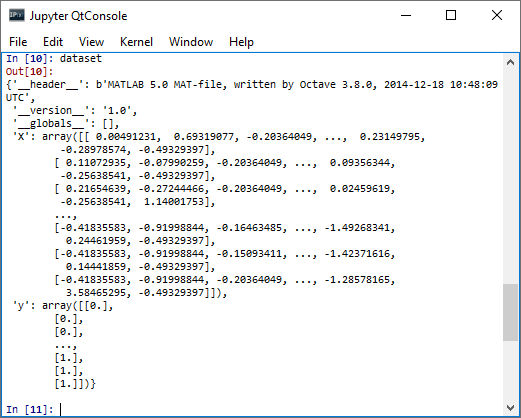
\includegraphics[scale=0.8]{imagenes/datasets_matlab}
	\caption{Contenido de los conjuntos de datos}
\end{figure}

Como podemos ver ``X'' contiene el conjunto de datos y el campo ``y'' contiene las etiquetas para los mismos.

En algunos de estos conjuntos de datos podemos encontrar lo que conocemos como valores perdidos o en inglés ``missing values''. Estos valores vienen reflejados con ``NAN'' en los conjuntos. Estos valores no sólo no nos son de interés si no que además nuestros modelos no están preparados para poder trabajar con ellos por lo que tenemos que decidir que transformación aplicamos para poder emplear los conjuntos de datos. La decisión tomada para estos valores ha sido la de eliminar las instancias que presenten valores perdidos. Esta decisión se basa en que, si estas instancias son anómalas no tenemos forma alguna de tratar con ellas porque no disponen de valores numéricos en sus campos y por tanto nuestros modelos no son aptos para resolver el conflicto. Esto no excluye el hecho de que estas instancias puedan ser anomalías reales. Por ejemplo pensemos en un sistema de frenos que sufre una rotura de alguno de sus sistemas. Si estos sistemas poseen sensores que recopilan datos es muy probable que estos sensores no tomen valores y por tanto dispongamos de valores perdidos precisamente porque la instancia es anómala. Esto se discutirá un poco más en profundidad cuando hablemos del trabajo futuro, de momento la decisión ha sido suprimir estas instancias.

Dentro de todos los conjuntos de datos que contiene la librería nosostros vamos a utilizar los siguientes:

\begin{table}[H]
	\begin{tabular}{|l|l|l|}
		\hline
		\multicolumn{1}{|c|}{{\ul \textbf{Nombre}}} & \multicolumn{1}{c|}{{\ul \textbf{Dimensionalidad}}} & \multicolumn{1}{c|}{{\ul \textbf{Número de instancias}}} \\ \hline
		annthyroid                                  & 6                                                   & 7200                                                     \\ \hline
		arrhythmia                                  & 274                                                 & 452                                                      \\ \hline
		breastw                                     & 9                                                   & 683                                                      \\ \hline
		cardio                                      & 21                                                  & 1831                                                     \\ \hline
		glass                                       & 9                                                   & 214                                                      \\ \hline
		ionosphere                                  & 33                                                  & 351                                                      \\ \hline
		letter                                      & 32                                                  & 1600                                                     \\ \hline
		lympho                                      & 18                                                  & 148                                                      \\ \hline
		mammography                                 & 6                                                   & 11183                                                    \\ \hline
		mnist                                       & 100                                                 & 7603                                                     \\ \hline
		musk                                        & 166                                                 & 3062                                                     \\ \hline
		optdigits                                   & 64                                                  & 5216                                                     \\ \hline
		pendigits                                   & 16                                                  & 6870                                                     \\ \hline
		pima                                        & 8                                                   & 768                                                      \\ \hline
		satellite                                   & 36                                                  & 6435                                                     \\ \hline
		satimage-2                                  & 36                                                  & 5803                                                     \\ \hline
		speech                                      & 400                                                 & 3686                                                     \\ \hline
		thyroid                                     & 6                                                   & 3772                                                     \\ \hline
		vertebral                                   & 6                                                   & 240                                                      \\ \hline
		vowels                                      & 12                                                  & 1456                                                     \\ \hline
		wbc                                         & 30                                                  & 378                                                      \\ \hline
		wine                                        & 13                                                  & 129                                                      \\ \hline
	\end{tabular}
\end{table}

Como podemos ver hay algunos conjuntos con un tamaño razonablemente grande tanto en dimensionalidad como en número de instancias. Esto será discutido modelo por modelo pues los algoritmos basados en subespacios tienen una complejidad dependiente del factorial de la dimensionalidad, es decir, a partir de una cierta dimensionalidad el tiempo que consumen estos algoritmos es demasiado alto.

\section{Experimentación}

Sobre estos conjuntos de datos hemos ejecutado nuestros cinco modelos implementados: HICS, OUTRES, Mahalanobis Kernel, Trinity y LODA. Sobre estas ejecuciones se ha recopilado el porcentaje de acierto sobre ellos, el tiempo consumido en la ejecución y las propias puntuaciones dadas sobre estos conjuntos de datos por los modelos.

Para poder hacer la comparativa con los datos de nuestros modelos he tomado modelos clásicos. Estos modelos se han cogido de la librería PyOD \cite{zhao_pyod:_2019}. De esta librería se han tomado 10 modelos: Angle-Based Outlier Detection (ABOD), Connectivity-Based Outlier Factor (COF), Histogram-Based Outlier Score (HBOS), K Nearest Neighbors (KNN), Local Outlier Factor (LOF), Minimum Covariance Determinant (MCD), One-Class Support Vector Machines (OCSVM), Principal Component Analysis (PCA), Subspace Outlier Detection (SOD) y Stochastic Outlier Selection (SOS). Sobre estos modelos se ha recopilado exactamente la misma información que sobre los nuestros, es decir, el acierto, el tiempo consumido y las puntuaciones de las instancias.

En cuanto a OUTRES podemos estudiar cuándo un subespacio es importante para una instancia completa. Por tanto hemos lanzado otro experimento para intentar analizar los subespacios que son más relevantes para una determinada instancia.

\section{Resultados}

En primer lugar vamos a ver los resultados que obtenemos de todos los modelos sobre todos los conjuntos de datos. Se muestra un gráfico de barras por cada conjunto de datos con el desempeño de cada modelo. Cabe decir que tanto OUTRES como HICS son algoritmos como hemos comentado con una eficiencia muy mala en tiempo. Al ser su complejidad en tiempo dependiente del factorial de la dimensionalidad sólo hemos ejecutado el algoritmo en conjuntos de datos de baja dimensionalidad para poder completar dicha ejecución en un tiempo razonable, aunque como veremos hay algunos conjuntos de datos cuya ejecución ha llevado varias horas.

Veamos primero todos los gráficos con los resultados para poder analizarlos y particularizar posteriormente.

\begin{figure}[H]
	\centering
	\label{annthyroid_accuracy}
	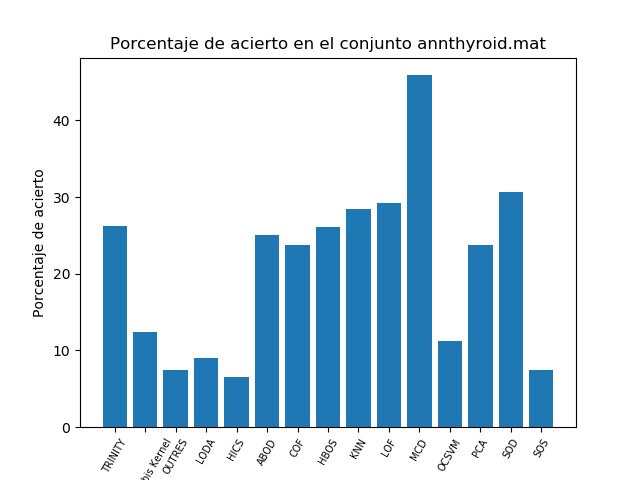
\includegraphics[scale=0.7]{imagenes/imgs-exp1/accuracy/annthyroid}
	\caption{Porcentaje de acierto sobre el conjunto de datos annthyroid}
\end{figure}

\begin{figure}[H]
	\centering
	\label{arrhythmia_accuracy}
	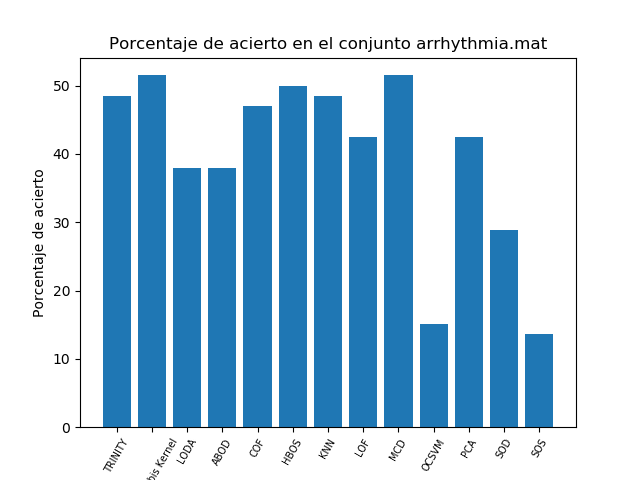
\includegraphics[scale=0.7]{imagenes/imgs-exp1/accuracy/arrhythmia}
	\caption{Porcentaje de acierto sobre el conjunto de datos arrhythmia}
\end{figure}

\begin{figure}[H]
	\centering
	\label{breastw_accuracy}
	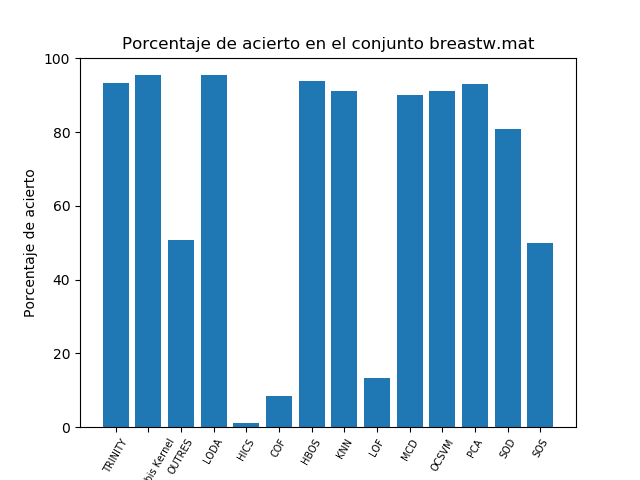
\includegraphics[scale=0.7]{imagenes/imgs-exp1/accuracy/breastw}
	\caption{Porcentaje de acierto sobre el conjunto de datos breastw}
\end{figure}

\begin{figure}[H]
	\centering
	\label{cardio_accuracy}
	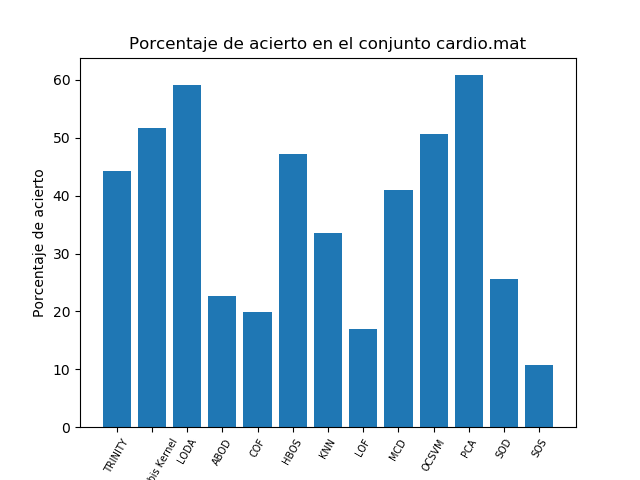
\includegraphics[scale=0.7]{imagenes/imgs-exp1/accuracy/cardio}
	\caption{Porcentaje de acierto sobre el conjunto de datos cardio}
\end{figure}

\begin{figure}[H]
	\centering
	\label{glass_accuracy}
	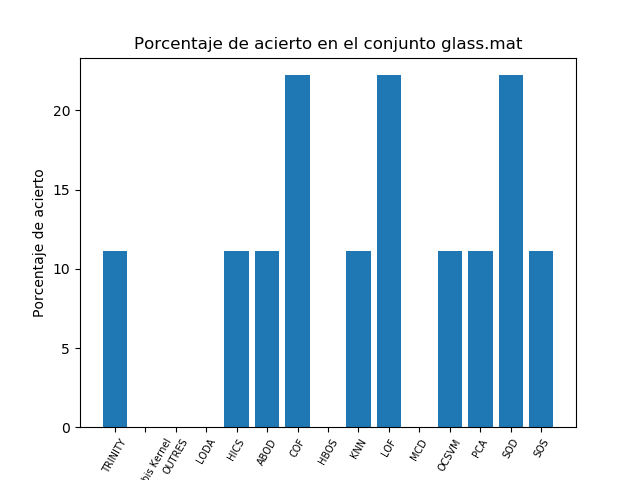
\includegraphics[scale=0.7]{imagenes/imgs-exp1/accuracy/glass}
	\caption{Porcentaje de acierto sobre el conjunto de datos glass}
\end{figure}

\begin{figure}[H]
	\centering
	\label{ionosphere_accuracy}
	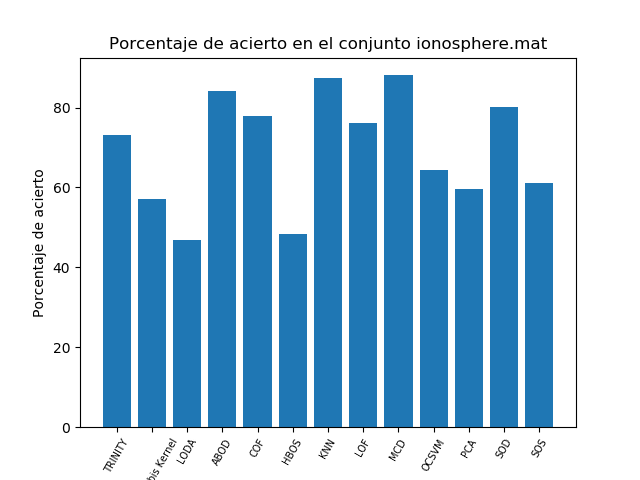
\includegraphics[scale=0.7]{imagenes/imgs-exp1/accuracy/ionosphere}
	\caption{Porcentaje de acierto sobre el conjunto de datos ionosphere}
\end{figure}

\begin{figure}[H]
	\centering
	\label{letter_accuracy}
	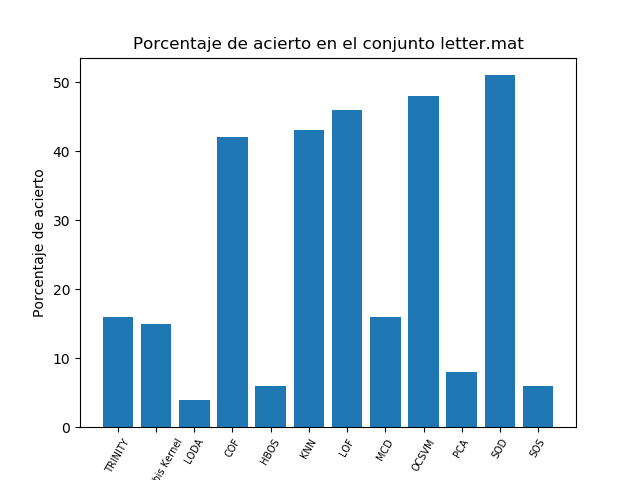
\includegraphics[scale=0.7]{imagenes/imgs-exp1/accuracy/letter}
	\caption{Porcentaje de acierto sobre el conjunto de datos letter}
\end{figure}

\begin{figure}[H]
	\centering
	\label{lympho_accuracy}
	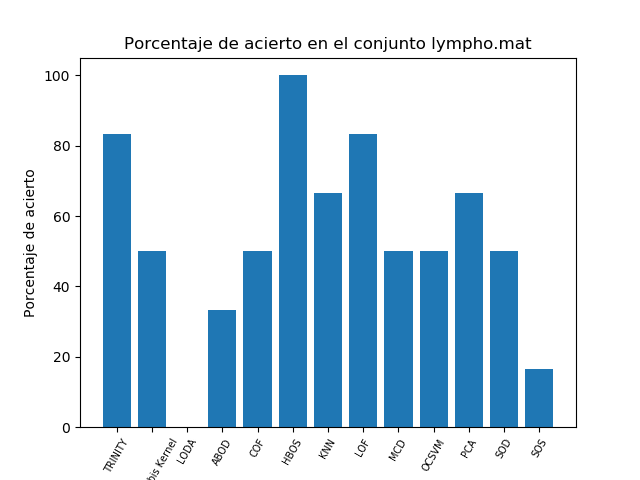
\includegraphics[scale=0.7]{imagenes/imgs-exp1/accuracy/lympho}
	\caption{Porcentaje de acierto sobre el conjunto de datos lympho}
\end{figure}

\begin{figure}[H]
	\centering
	\label{mammography_accuracy}
	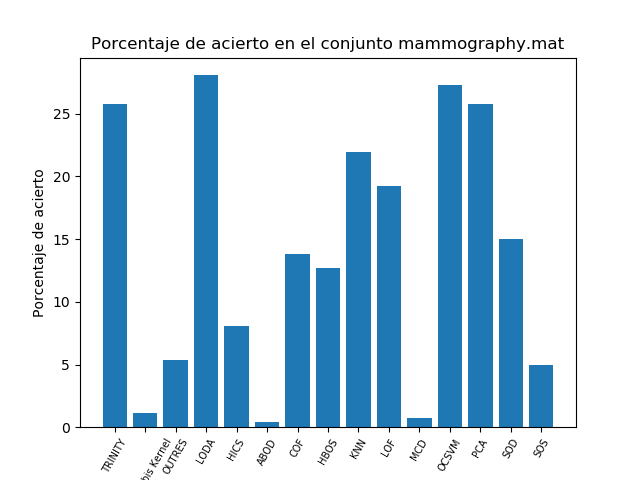
\includegraphics[scale=0.7]{imagenes/imgs-exp1/accuracy/mammography}
	\caption{Porcentaje de acierto sobre el conjunto de datos mammography}
\end{figure}

\begin{figure}[H]
	\centering
	\label{mnist_accuracy}
	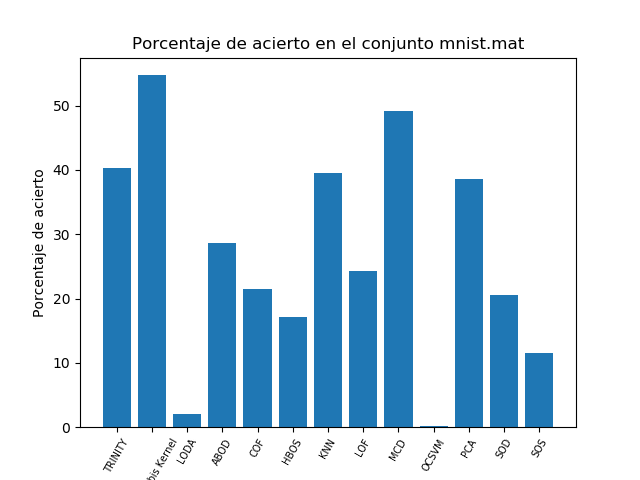
\includegraphics[scale=0.7]{imagenes/imgs-exp1/accuracy/mnist}
	\caption{Porcentaje de acierto sobre el conjunto de datos mnist}
\end{figure}

\begin{figure}[H]
	\centering
	\label{musk_accuracy}
	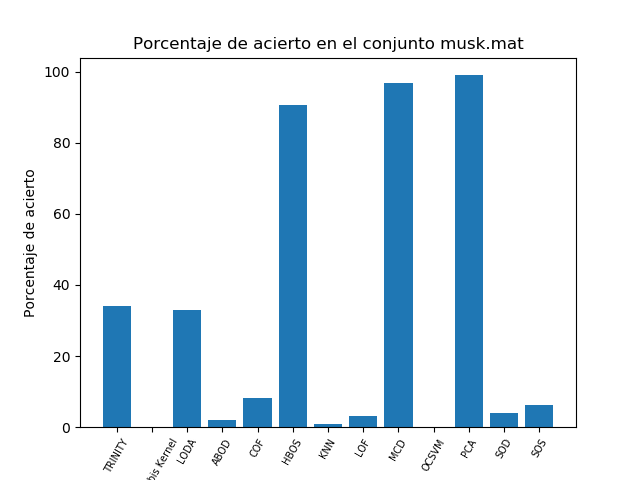
\includegraphics[scale=0.7]{imagenes/imgs-exp1/accuracy/musk}
	\caption{Porcentaje de acierto sobre el conjunto de datos musk}
\end{figure}

\begin{figure}[H]
	\centering
	\label{optdigits_accuracy}
	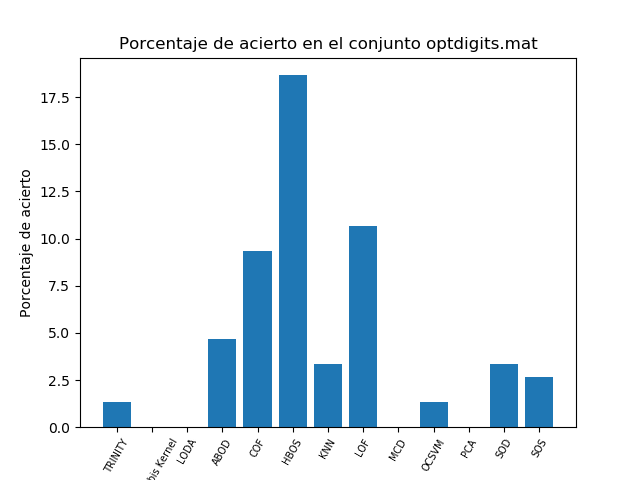
\includegraphics[scale=0.7]{imagenes/imgs-exp1/accuracy/optdigits}
	\caption{Porcentaje de acierto sobre el conjunto de datos optdigits}
\end{figure}

\begin{figure}[H]
	\centering
	\label{pendigits_accuracy}
	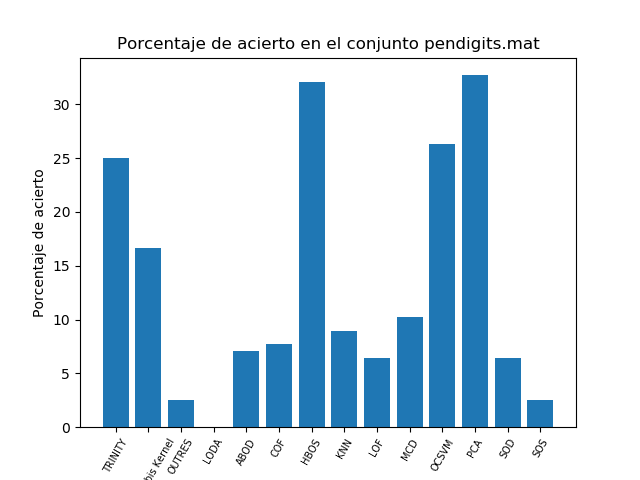
\includegraphics[scale=0.7]{imagenes/imgs-exp1/accuracy/pendigits}
	\caption{Porcentaje de acierto sobre el conjunto de datos pendigits}
\end{figure}

\begin{figure}[H]
	\centering
	\label{pima_accuracy}
	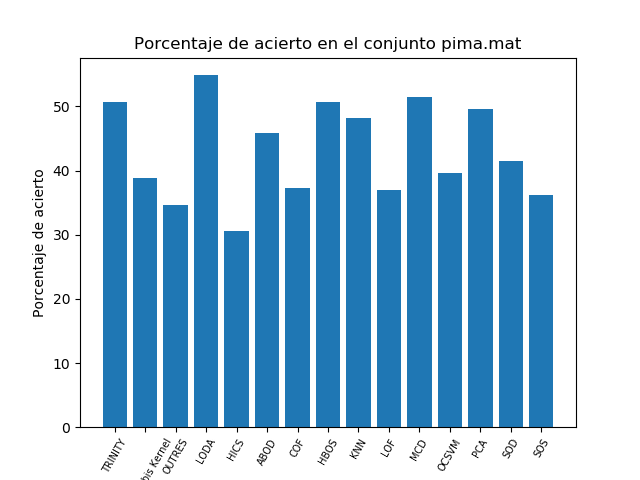
\includegraphics[scale=0.7]{imagenes/imgs-exp1/accuracy/pima}
	\caption{Porcentaje de acierto sobre el conjunto de datos pima}
\end{figure}

\begin{figure}[H]
	\centering
	\label{satellite_accuracy}
	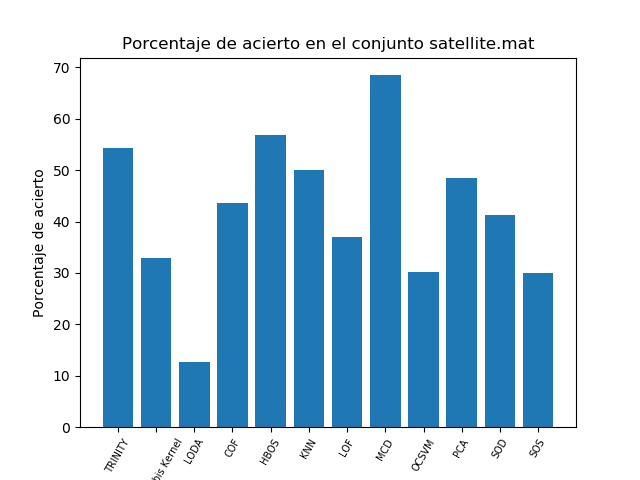
\includegraphics[scale=0.7]{imagenes/imgs-exp1/accuracy/satellite}
	\caption{Porcentaje de acierto sobre el conjunto de datos satellite}
\end{figure}

\begin{figure}[H]
	\centering
	\label{satimage-2_accuracy}
	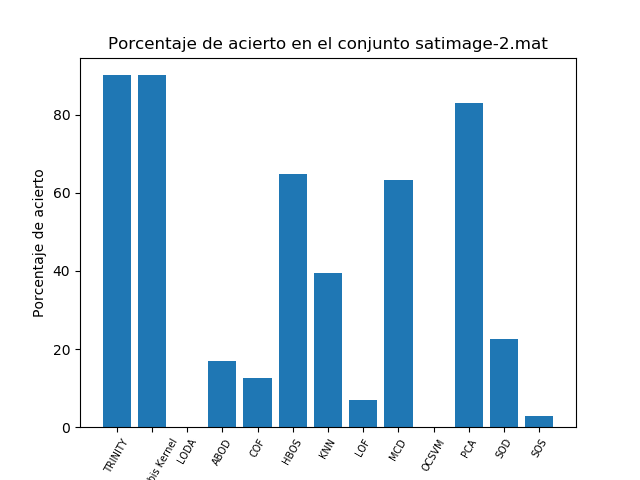
\includegraphics[scale=0.7]{imagenes/imgs-exp1/accuracy/satimage-2}
	\caption{Porcentaje de acierto sobre el conjunto de datos satimage-2}
\end{figure}

\begin{figure}[H]
	\centering
	\label{speech_accuracy}
	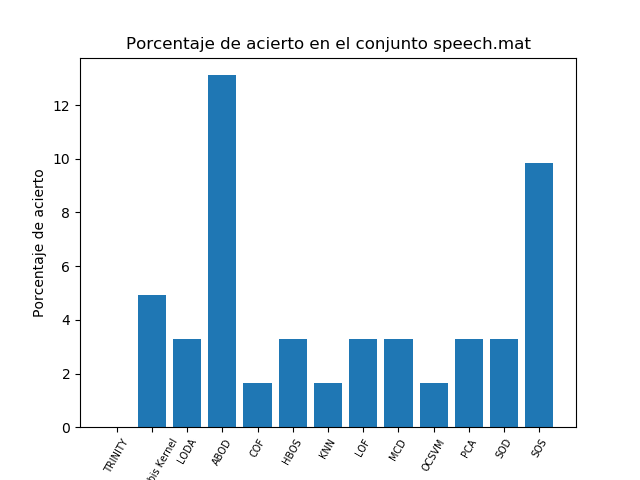
\includegraphics[scale=0.7]{imagenes/imgs-exp1/accuracy/speech}
	\caption{Porcentaje de acierto sobre el conjunto de datos speech}
\end{figure}

\begin{figure}[H]
	\centering
	\label{thyroid_accuracy}
	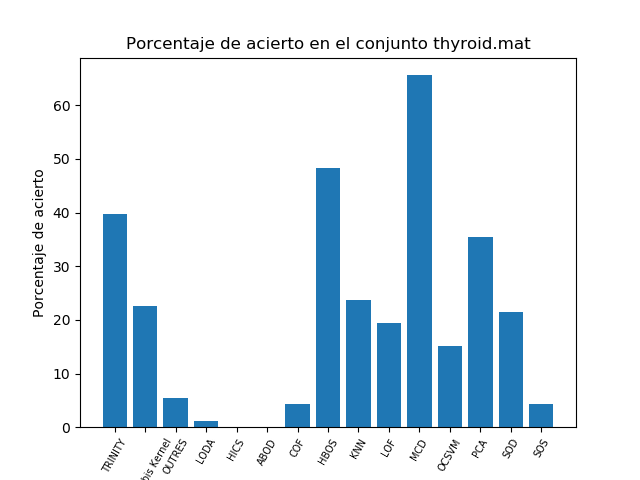
\includegraphics[scale=0.7]{imagenes/imgs-exp1/accuracy/thyroid}
	\caption{Porcentaje de acierto sobre el conjunto de datos thyroid}
\end{figure}

\begin{figure}[H]
	\centering
	\label{vertebral_accuracy}
	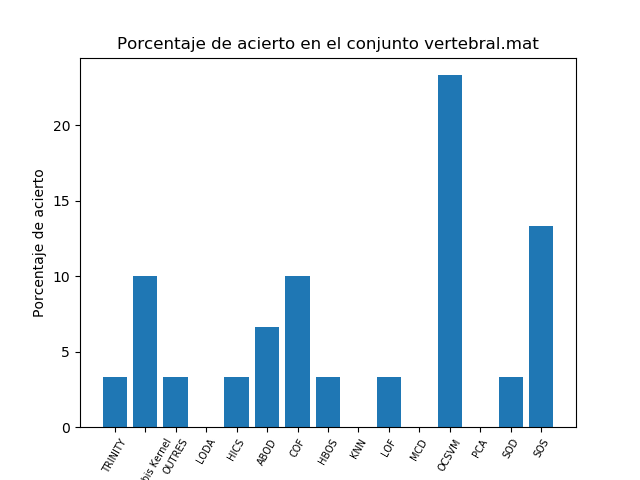
\includegraphics[scale=0.7]{imagenes/imgs-exp1/accuracy/vertebral}
	\caption{Porcentaje de acierto sobre el conjunto de datos vertebral}
\end{figure}

\begin{figure}[H]
	\centering
	\label{vowels_accuracy}
	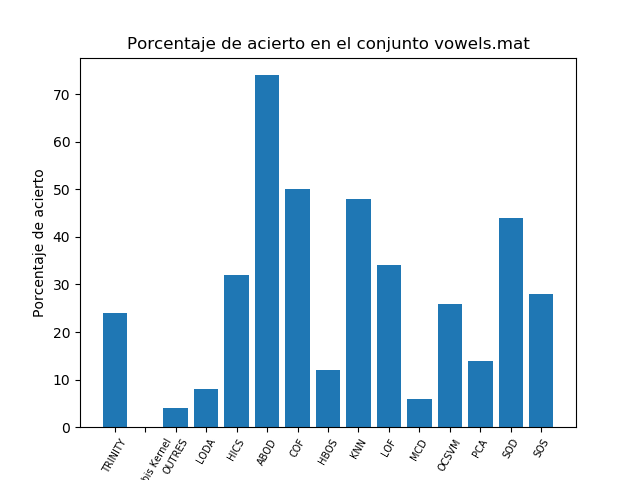
\includegraphics[scale=0.7]{imagenes/imgs-exp1/accuracy/vowels}
	\caption{Porcentaje de acierto sobre el conjunto de datos vowels}
\end{figure}

\begin{figure}[H]
	\centering
	\label{wbc_accuracy}
	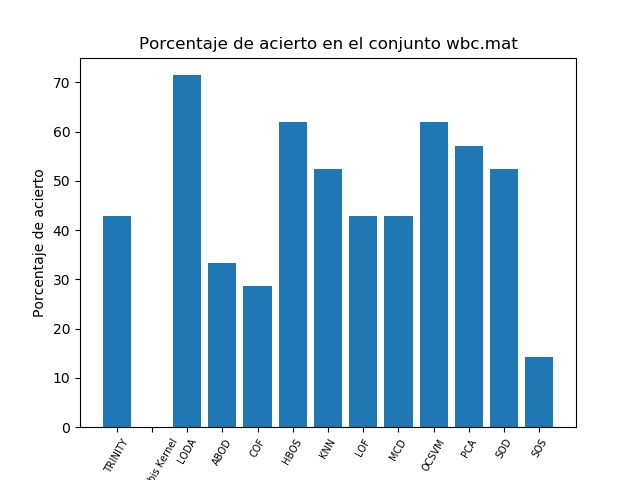
\includegraphics[scale=0.7]{imagenes/imgs-exp1/accuracy/wbc}
	\caption{Porcentaje de acierto sobre el conjunto de datos wbc}
\end{figure}

\begin{figure}[H]
	\centering
	\label{wine_accuracy}
	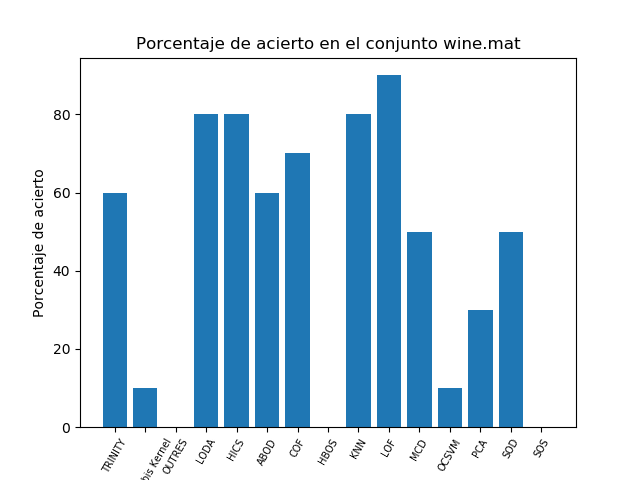
\includegraphics[scale=0.7]{imagenes/imgs-exp1/accuracy/wine}
	\caption{Porcentaje de acierto sobre el conjunto de datos wine}
\end{figure}

Como podemos observar los resultados que hemos obtenido han sido variados. En primer lugar cabe justificar algunos valores en función de la dificultad de la tarea. Como hemos comentado en la parte teórica el concepto de anomalía es algo difícil de enmarcar por lo que también es algo complejo de detectar y por tanto en función de cada conjunto de datos puede que detectemos mejor o peor sus anomalías. Por eso por ejemplo tenemos conjuntos de datos como \ref{glass_accuracy} en los que el mejor de los resultados apenas es poco más de un 20\% o \ref{optdigits_accuracy} en el que ni siquiera llegamos a dicho 20\%. Esto no es más que el reflejo de la dificultad del problema. Lo interesante de este estudio es si conseguimos mejorar en algún caso con respecto a los modelos tradicionales y la respuesta es que alguno de los modelos que hemos implementado superan en ciertos conjuntos de datos a los clásicos.

Hemos conseguido con nuestros modelos conseguir la mejor puntuación en $8$ de $22$ conjuntos de datos. Este resultado puede no parecer significativo pero debemos considerar que tenemos el doble de modelos clásicos que de modelos de ensamblaje y que ni mucho menos todos los algoritmos clásicos están al mismo nivel. Además tenemos algoritmos clásicos de todos los tipos por lo que como podemos ver en algunos conjuntos de datos no funcionan todos bien pero alguno destaca y viceversa. 

Como podemos ver en los $22$ conjuntos de datos que hemos probado los dos modelos que peores resultados nos han arrojado de loa 5 implementados son HICS y OUTRES, es decir, los dos modelos basados en subespacios que hemos implementado. Esto no quiere decir que los dos modelos sean de poca relevancia. Creo que la idea del estudio por subespacio es algo razonable y que puede arrojar buenos resultados, pero quizás no hemos utilizado para estos dos algoritmos ningún conjunto de datos conveniente. Además creo que los algoritmos de subespacios presentados son un poco rígidos en esta concepción sin querer salirse de la misma. Por ejemplo HICS obtiene sobre todo según hemos  visto anomalías que no son triviales o claramente basadas en la definición de distancias. Es por esto que, aunque lo hayamos probado como un modelo sólo, pienso que es un algoritmo más idóneo para aplicarlo en conjunción con otro tipo de algoritmos. Por ejemplo sería interesante aplicar un algoritmo basado en subespacios después de aplicar Mahalanobis Kernel puesto que este modelo y Trinity son los más fiables de los 5 que hemos estudiado. Por ejemplo podemos ver que en \ref{arrhythmia_accuracy}, \ref{breastw_accuracy}, \ref{mnist_accuracy} o \ref{satimage-2_accuracy} tanto Trinity como Mahalanobis Kernel funcionan muy bien. 

Hay un dato bastante interesante en la comparativa entre Mahalanobis Kernel y Trinity. Como hemos visto en la explicación de los modelos Trinity tiene a Mahalanobis Kernel en el primer componente. Esto en los resultados se refleja en que Trinity en general obtiene mejores resultados que Mahalanobis Kernel. El segundo componente vimos que era KNN, comparando con este modelo vemos que los resultados que obtiene Trinity son al menos iguales aunque en varios conjuntos son mejores los de Trinity que los de KNN. Por último el tercer componente de Trinity es IForest que no ha entrado dentro de esta comparativa por ser un modelo de ensamblaje también y por tanto carece de sentido contraponerlo con nuestros modelos. Esto nos está mostrando que efectivamente la combinación de modelos hace que los resultados sean más robustos obteniendo mejores resultados en general o en el peor caso manteniendo aproximadamente los resultados del modelo individual.

Por último podemos ver que LODA en general no tiene unos resultados muy espectaculares. Aún así consigue ponerse en cabeza en \ref{breastw_accuracy}, \ref{cardio_accuracy}, \ref{mammography_accuracy}, \ref{pima_accuracy} y \ref{wbc_accuracy}. En el resto de conjuntos de datos no obtiene unos buenos resultados, lo que nos está diciendo que funciona muy bien en conjuntos de datos adecuados.

Vamos a ver ambos conjuntos de datos para comprobar la razón de este comportamiento.

\begin{figure}[H]
	\centering
	\label{breastw}
	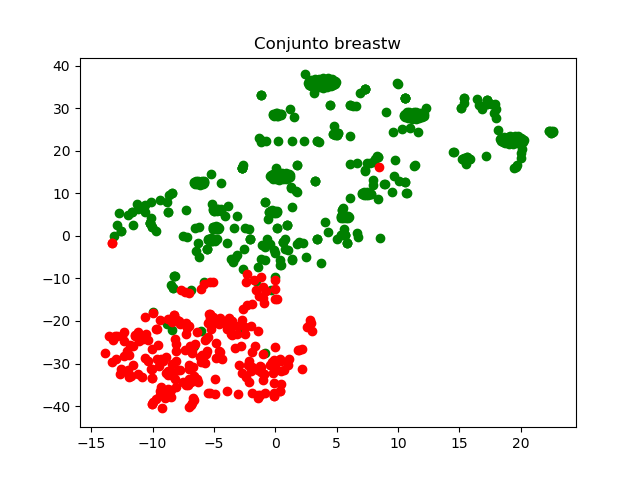
\includegraphics[scale=0.7]{imagenes/breastw}
	\caption{Proyección de breastw}
\end{figure}

\begin{figure}[H]
	\centering
	\label{glass}
	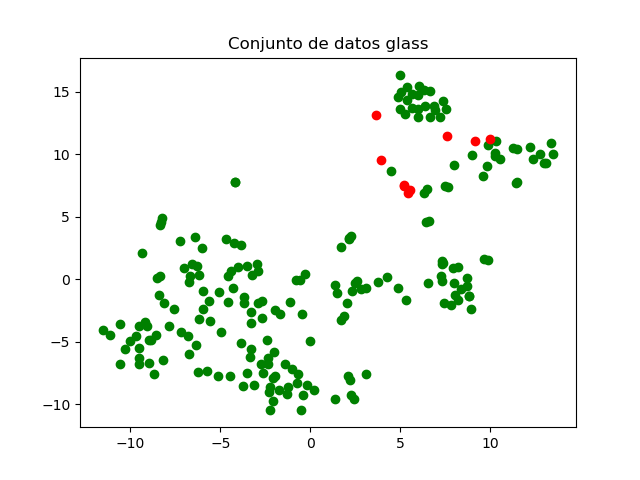
\includegraphics[scale=0.7]{imagenes/glass}
	\caption{Proyección de glass}
\end{figure}

Como podemos ver en las figuras primeras LODA funciona muy bien sobre el conjunto de datos breastw y muy mal sobre el conjunto de datos glass. Para comprobar la forma de estos dos conjuntos de datos hemos dibujado la proyección en dos dimensiones utilizando la técnica TSNE. Como podemos observar en el conjunto de datos breastw tenemos las anomalías muy separadas del resto de los datos (siendo las anomalías los datos en rojo) mientras que en glass están dentro de los datos que consideraríamos normales. Esto nos está diciendo que cuanto mayor sea la aparición de anomalías del tipo basadas en distancias mejor es el desempeño de LODA. 

Como podemos ver casi todos los modelos fallan en conjuntos de datos como optdigits. Veamos su proyección para intentar entenderlo.

\begin{figure}[H]
	\centering
	\label{optdigits}
	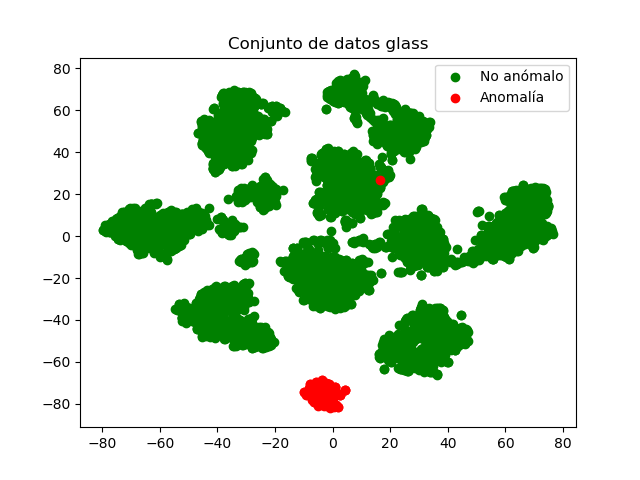
\includegraphics[scale=0.7]{imagenes/optdigits}
	\caption{Proyección de optdigits}
\end{figure}

Podría parecer que el mal desempeño de los algoritmos sea completamente ilógico al ver que las anomalías están completamente diferenciadas de los datos. Como podemos ver no sólo están separadas del resto de los datos, si no que además están muy apiñadas entre sí. Esto es un inconveniente tremendo en la detección de anomalías. Como vimos en la primera de las definiciones las anomalías deben ser datos cuya distancia al centroide sea alta cosa que no pasa en este conjuntos de datos. Si nos fijamos en la segunda definición estamos intentando estudiar la densidad de datos para ver la anomalía pero este cluster tiene una alta densidad con lo que los datos no entrarían en la definición. Este conjunto de datos refleja perfectamente la complejidad del problema. Tenemos empíricamente determinadas las anomalías pero no entran claramente en las definiciones que podemos proveer de las mismas con lo que nos es difícil clasificarlas.

HICS tiene un desempeño razonablemente bueno en el conjunto de datos wine con lo que vamos a ver su proyección e intentar sacar conclusiones.

\begin{figure}[H]
	\centering
	\label{wine}
	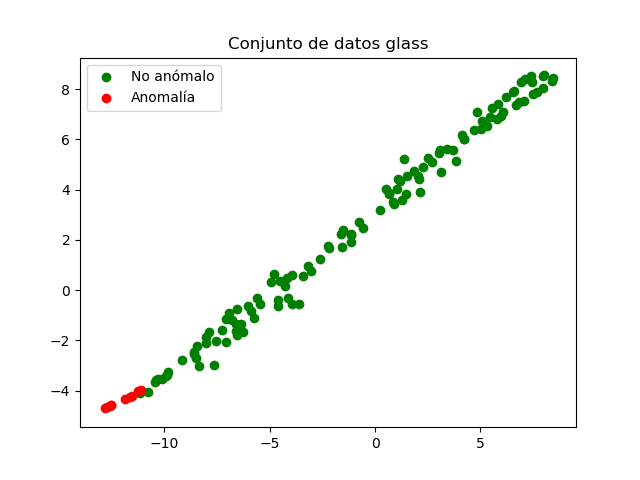
\includegraphics[scale=0.7]{imagenes/wine}
	\caption{Proyección de wine}
\end{figure}

La proyección nos está mostrando que los datos están esparcidos a lo largo de un eje con lo que podemos explicar perfectamente también el buen desempeño de Mahalanobis Kernel. En concreto podemos deducir que HICS entiende que estos datos son anómalos o al menos más anómalos que el resto de los datos porque tienen una menor densidad en su entorno. Claramente es el punto en el que menos datos hay alrededor por lo que podemos ver razonable el comportamiento satisfactorio de HICS.

Para comprender el comportamiento de outres es buena idea comprobar no sólo cuándo tenemos buenos resultados, si no que además por el propio algoritmo podemos ver el subespacio de los datos en el que cada dato es anómalo.

OUTRES no obtiene demasiados resultados satisfactorios pero donde mejor funciona es en breastw y en pima. Ya hemos visto cómo es la proyección de breastw, veamos la de pima.

\begin{figure}[H]
	\centering
	\label{wine}
	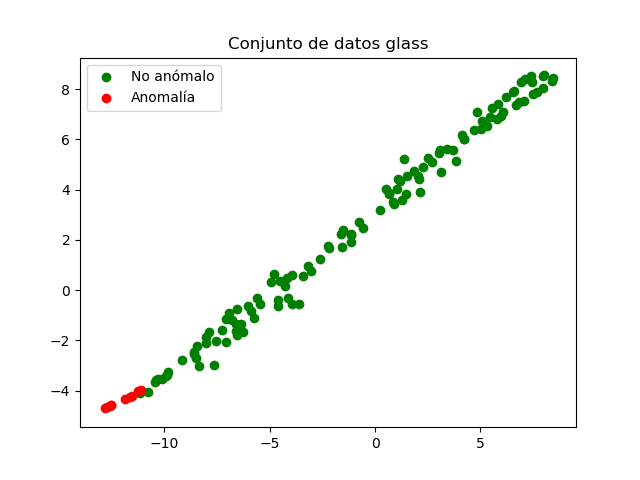
\includegraphics[scale=0.7]{imagenes/wine}
	\caption{Proyección de wine}
\end{figure}
